\section{Objectives}
Follow Lab 6 (PDF pages 24--25) to compare real MOS input loading with the handout's 8/16/24/32 fF fixed-capacitance approximations.

\section{Specification mapping}
\begin{longtable}{p{0.31\linewidth}p{0.29\linewidth}p{0.31\linewidth}}
\toprule
Handout requirement (PDF page) & Implementation & Verification and scope \\\midrule
Step 1: four Table 6.1 cases (24--25) & 01\_gate\_load: NL=1--4 & All four cases simulated \\
Compare MOS and fixed-C waveform/delay (25) & 8 fF per doubled MLOAD & Differences quantified; equality not assumed \\
\bottomrule
\end{longtable}


\section{Circuit and design derivation}
Both drivers use $W_n=0.6\,\mu$m, $W_p=1.8\,\mu$m and $L=0.25\,\mu$m. Each MOS load doubles the widths to $1.2/3.6\,\mu$m. NL identical loads connect in parallel to the same driver output; MOS multiplicity represents these parallel units while their output still switches. The reference case a used a unit load, and case b cascaded loads. Both are corrected to the doubled parallel loading specified in the handout.

The estimate is $C_g\approx C_{ox}(W_n+W_p)L$, with $C_{ox}=\epsilon_{ox}/t_{ox}$. The handout's 5.4 nm oxide gives about 7.87 fF per load only for its original process. The supplied encrypted model does not expose a verified oxide thickness. The handout's prose reverses W/L labels; W denotes width and L length here.

\section{Simulation setup}
This teaching rewrite uses a separately supplied model at 1.0 V and $25\,^{\circ}\mathrm C$. The specified topology, loads and comparative dimensions are retained. The handout's 2.5 V process results are not acceptance values for this model. The chosen 1 V is a simulation condition, not a verified device rating. MOS bulk terminals are explicitly connected to the corresponding supply rails.

HSPICE S-2021.09 uses RUNLVL=6, retaining waveforms, printed data and native measurements. Figures are redrawn from actual data; CSV files are in each Lab's results directory. Successful solution does not establish process reliability. Warnings from encrypted model blocks remain suppressed; the existing diagnostic did not expose actionable further details, so the warnings are not declared harmless and complete model-limit compliance is not claimed.

Input edges are 0.1 ns with a 5 ns period; transient duration is 10 ns with 1 ps printing. Both output 10--90\% transitions and input/output 50\% propagation delays are measured.

\section{Results and specification checks}
All four cases solved and measured successfully. Delays below are in ps; MOS/C denote real loads/fixed capacitors.
\begin{center}\small
\begin{tabular}{llllll}
\toprule
NL & $C$ (fF) & $t_{pHL,MOS}$ & $t_{pHL,C}$ & $t_{pLH,MOS}$ & $t_{pLH,C}$ \\
\midrule
1 & 8 & 76.80 & 63.82 & 139.95 & 88.76 \\
2 & 16 & 112.89 & 85.88 & 241.42 & 127.05 \\
3 & 24 & 148.64 & 107.34 & 339.83 & 164.48 \\
4 & 32 & 184.10 & 128.38 & 439.90 & 201.64 \\
\bottomrule
\end{tabular}
\end{center}

\begin{figure}[htbp]
\centering
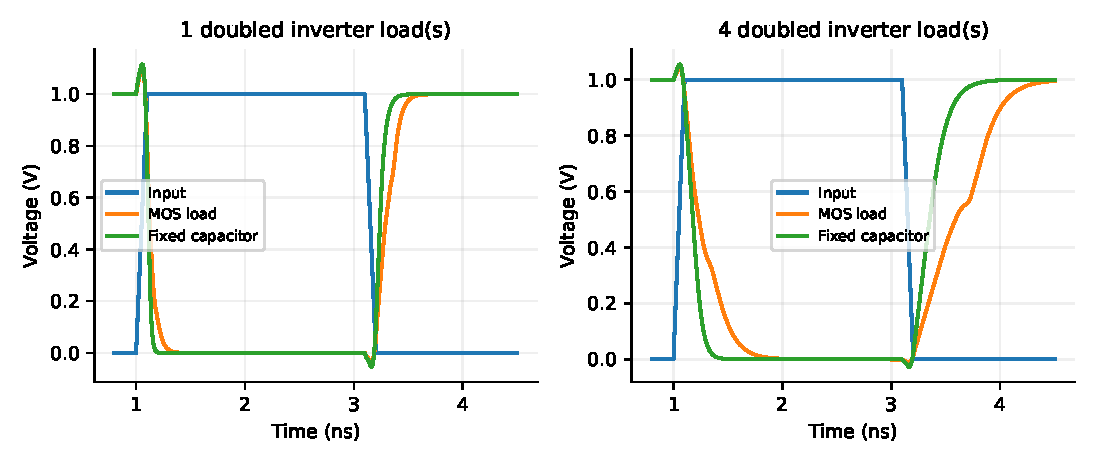
\includegraphics[width=\linewidth]{figures/gate_load_waveforms.pdf}
\caption{Waveforms with one and four loads; redrawn from this run's HSPICE data.}
\end{figure}

\begin{figure}[htbp]
\centering
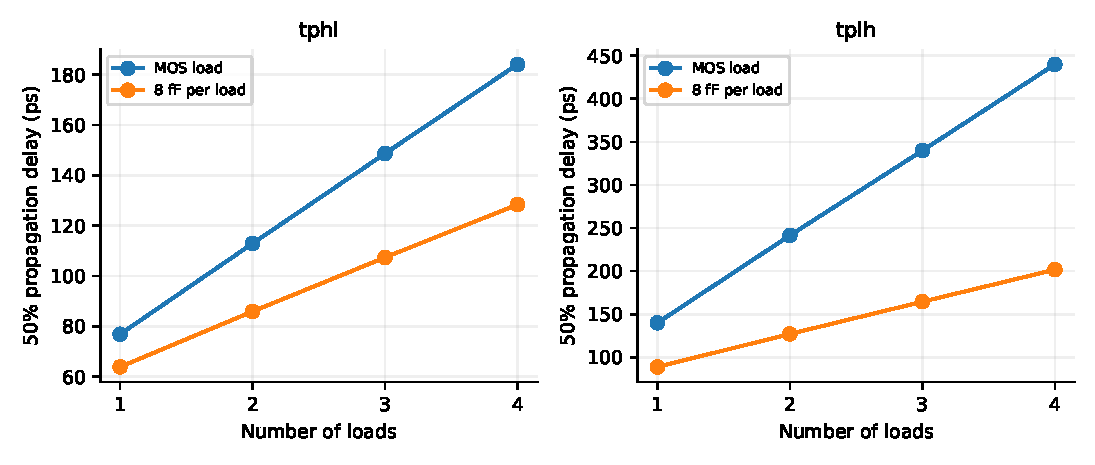
\includegraphics[width=\linewidth]{figures/gate_load_delays.pdf}
\caption{Propagation delay for the two load models; redrawn from this run's HSPICE data.}
\end{figure}


\section{Discussion}
The real MOS load is slower than the handout's fixed capacitor in all four cases, particularly for charging: NL=4 gives 439.90 ps versus 201.64 ps with 32 fF. Gate capacitance, overlap/Miller coupling and movement of the load output contribute; a single $C_{ox}WL$ value cannot capture every state. The handout's approximate equality is not reproduced under this model, a documented process-adaptation difference rather than an omitted experiment.

\section{Conclusion}
All four requested comparisons are complete. Eight fF per load is not a validated equivalent for this model. A subsequent cell-library model would require fitting across input slew, output loading and logic state.
